\documentclass[12pt,a4paper]{article}
\usepackage[utf8]{inputenc}
\usepackage[russian]{babel}
\usepackage[OT1]{fontenc}
\usepackage{graphicx}
\usepackage{calc}
\usepackage[margin=15mm]{geometry}
\usepackage{cmap}

% условие без картинки
\newcommand{\task}[2]{
\hrule
\hbox to \textwidth {%
     \vrule
\parbox[t]{0.04\textwidth}{\smallskip \centering #1}%
     \vrule%
\hfill%
     \parbox[t]{0.93\textwidth}{\smallskip #2 \smallskip}\hfill%
\vrule
}
\hrule
    \pagebreak[2]
}

\newlength{\h}
\newsavebox{\taskbox}
\newlength{\x}
\newsavebox{\pictbox}

% условие с картинкой (картинка выравнивается по центру)
\newcommand{\taskpic}[3]{
\savebox{\taskbox}{\parbox[t]{0.93\textwidth-4.3cm}{\smallskip #2 \smallskip}}
\savebox{\pictbox}{\parbox[t]{4cm}{\smallskip \centering
     \vspace{0pt} #3 \smallskip}}
\h=\ht\taskbox
\advance\h\dp\taskbox
\x=\ht\pictbox
\advance\x\dp\pictbox
\hrule
\hbox to \textwidth {%
\vrule\parbox[t][\maxof{\h}{\x}][t]{0.04\textwidth}{ \smallskip
     \centering #1 }\vrule%
\hfill\parbox[t][\maxof{\h}{\x}][t]{0.93\textwidth-4.3cm}{\smallskip #2
     \smallskip}\hfill\vrule%
\hfill\parbox[t][\maxof{\h}{\x}][c]{4cm}{\hfil #3 \hfil}\hfill\vrule
}
\hrule
\pagebreak[2]
}
\pagestyle{empty}
\graphicspath{ {images/} }

\begin{document}

\begin{center}
\begin{Large}
\textsc{ГЦФО. 9 класс. 2014/15.}
\end{Large}
\end{center}

\task{29}{На гладком горизонтальном столе лежат два одинаковых бруска, соединенных пружиной жесткости $k$ и длины $l_0$. На левый брусок внезапно начинает действовать постоянная сила $F$, направленная вдоль пружины. Найдите минимальное и максимальное расстояние между брусками.}
\task{31}{Локомотив с постоянной силой тяги $F$ начал двигаться к стоящему вагону и столкнулся с ним через время $\Delta t$. Найдите время между последующими соударениями локомотива с этим вагоном. Удар упругий. Трением в осях колес пренебречь. Массы вагона и локомотива не одинаковы.}
\taskpic{34}{На концах длинной нити подвешены грузы массы $m$ каждый. Нить перекинута через два легких маленьких блока, расположенных на расстоянии $2l$ друг от друга. К ней посередине между блоками прикрепляют груз массы $2m$, и система приходит в движение. Найдите скорость грузов по истечении достаточно большого промежутка времени.}{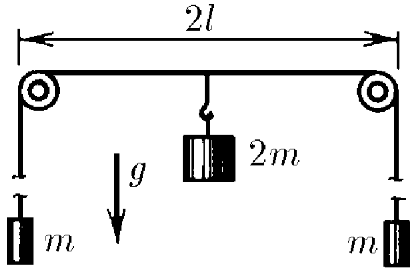
\includegraphics[width=4cm]{34}}
\taskpic{35}{Деревянная и металлическая однородные балки соединены, как показано на рисунке. Размеры, указанные на рисунке, составляют $a=10$ см, $b=5$ см, $c=35$ см. Темным цветом изображена металлическая балка. Известно, что вся конструкция может плавать, полностью погрузившись в воду. Какой угол при этом составляет длинная балка с вертикалью?}{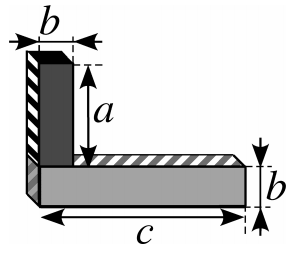
\includegraphics[width=4cm]{35}}
\taskpic{36}{Из однородной проволоки спаяли схему, состоящую из колец (см. рис.). Внешнее кольцо имеет диаметр $D$, внутрь него вложены два кольца вдвое меньшего диаметра; в каждое из меньших колец вложены еще два, которые меньше еще вдвое. В местах касания колец есть электрический контакт. Клемма Ф присоединена к середине дуги правой полуокружности. Найдите сопротивление этой схемы между клеммами Д и Ф. Каким будет сопротивление схемы, в которой кольца из проволоки вкладываются по данному правилу до бесконечности? Сопротивление единицы длины проволоки $\lambda$.}{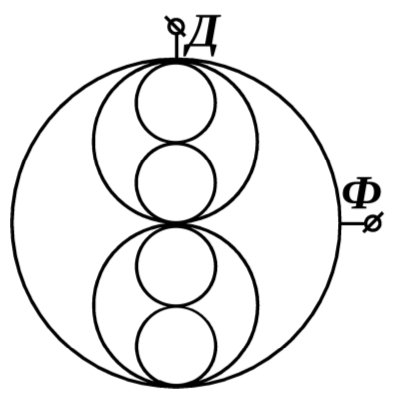
\includegraphics[width=4cm]{36}}
\taskpic{37}{Труба, сечение которой является квадратом со стороной $a = 20$ см, закрыта поршнем. К трубе присоединена вертикальная трубка. Часть трубы, находящаяся справа от поршня, полностью заполнена водой. Чтобы удерживать поршень в равновесии, к нему необходимо прикладывать силу $F = 16$ Н, направленную вправо. Каков уровень воды в трубке? Плотность воды $\rho = 1000$ кг/м$^3$, ускорение свободного падения $g = 10$ м/с$^2$. Трение отсутствует.}{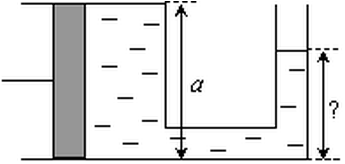
\includegraphics[width=4cm]{37}}

\end{document}
